% Recuperato senza modifiche dal commit c408be9.
% Sorgente: chapters/04_forme_differenziali/02_multilineari.tex
\documentclass[tikz,border=5pt]{standalone}
\usepackage{amsmath}
\usetikzlibrary{arrows.meta}
\begin{document}
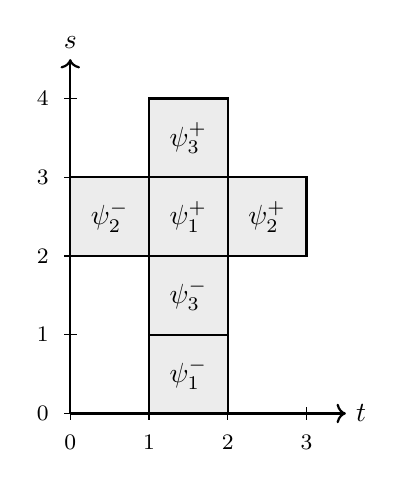
\begin{tikzpicture}[scale=1]
  % disegno dei 6 quadrati dello sviluppo del cubo (coordinate intere non negative)
  % posizione dei quadrati: (1,2) centro, sopra (1,3), sinistra (0,2), destra (2,2), sotto (1,1), sotto2 (1,0)
  \foreach \x/\y/\lab in {1/2/$\psi_1^+$,1/3/$\psi_3^+$,0/2/$\psi_2^-$,2/2/$\psi_2^+$,1/1/$\psi_3^-$,1/0/$\psi_1^-$} {
    \fill[gray!15] (\x,\y) rectangle ++(1,1);
    \draw[thick] (\x,\y) rectangle ++(1,1);
    \node at (\x+0.5,\y+0.5) {\lab};
  }
  % assi coordinati con etichette t (asse x) e s (asse y)
  \draw[->, thick] (0,0) -- (3.5,0) node[right] {$t$};
  \draw[->, thick] (0,0) -- (0,4.5) node[above] {$s$};
  \foreach \i in {0,1,2,3} {\draw (\i,0.08) -- (\i,-0.08) node[below,yshift=-2pt] {\footnotesize \i};}
  \foreach \j in {0,1,2,3,4} {\draw (0.08,\j) -- (-0.08,\j) node[left,xshift=-2pt] {\footnotesize \j};}
\end{tikzpicture}
\end{document}
